\cleardoublepage
\chapter{文献综述}

\section{背景介绍}
\par 宫颈癌是女性第四常见的癌症类型,严重威胁着女性的生命和健康。2018年,全球估计有57万女性被诊断出患有宫颈癌,约31.1万女性死于该疾病。然而,宫颈癌是缓慢增长的,从癌前病变到病发的时间在5年或更长,这为通过早期发现和适当治疗降低宫颈癌的发病率和死亡率提供了机会。全世界大约七成的宫颈癌发生在发展中国家\cite{wild2014world},在发达国家中,因为宫颈抹片筛查以及其他检测方法的普及,宫颈癌的发病率和致死率大大降低\cite{canavan2000cervical}。这也说明,定期进行科学的宫颈癌筛查是十分必要的。
\par 宫颈癌筛查主要由“细胞学-阴道镜-组织学”三阶梯诊断程序组成,其中,细胞学筛查的主要手段就是TCT检查,即采用液基薄层细胞检测系统检测宫颈细胞并进行细胞学分类诊断。TCT检查需要医生使用专门的宫颈刷来采集子宫颈的脱落细胞样本,再将细胞样本漂洗后转移到保存液瓶中,然后放入全自动细胞检测仪中将细胞混匀、过滤、转移,并最后将细胞帖附到玻片上。之后需要将玻片进行染色固定才能在显微镜下通过估计细胞的类型和形态特征,如细胞核大小、核胞浆比进行观察诊断,最后按照Bethesda系统(TBS)的描述性诊断方法给出诊断报告。
\par 宫颈TCT筛查通常需要医生通过显微镜在整个玻片上寻找疑似病变或病变细胞,最后根据全片病变细胞的状况给出诊断。但是,在医生阅片的过程中可能会遇到许多问题。

\begin{enumerate}
    \item TCT阅片耗时费力
          \par 如\ref{全片}所示,整个TCT样本的片子含有几亿甚至几十亿像素,十分巨大。玻片上也有上亿细胞,数目非常多。检阅全片需要非常大的工作量。由此,在临床实践中可能会遗漏病变细胞,从而影响诊断结果的准确性。例如,如果医生在阅片时遗漏了某个病变等级较高的细胞聚集的区域,那么诊断结果可能会更倾向于较低的病变等级,这显然不利于医生做出准确的诊断结果也不利于医生和患者获悉正确的病情。而且,这一过程使得诊断结果具有了一定的随机性,使其不能准确描述患者的病情。

          \begin{figure}[h]
              \centering
              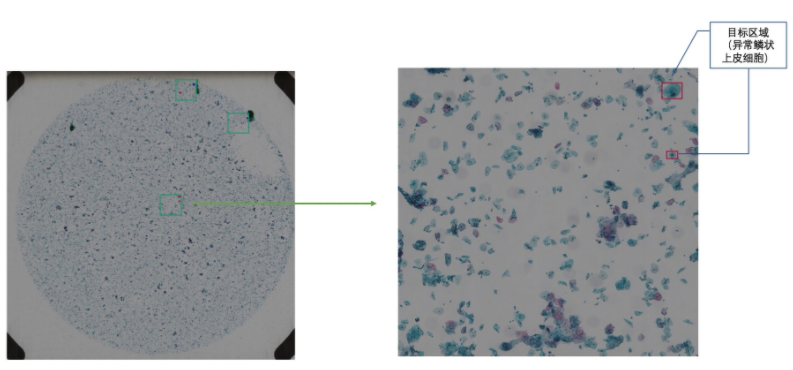
\includegraphics[width=0.5\paperwidth]{TCT/whole_pic.png}
              \caption{全片与部分视野的大小对比。左图为全片,右图为一个视野,在视野中可以看到正常细胞与病变细胞}
              \label{全片}
          \end{figure}
    \item 类别判定的主观性
          \par 此外,全人工的阅片可能会导致诊断结果的主观性过强,某些类别的判定可能没有十分明确的标准导致医生在诊断时诊断结果取决于医生的主观偏好。以\ref{HSIL-SQCA}为例,可以看到右图中部分被标注为HSIL的病变区域有着与SQCA区域几乎相同的形态特征而与左图中的HSIL类别的形态差异较大。这是因为在临床实践中,SQCA类别的检出更依赖于组织病理切片而不是TCT检查,所以医生在判定这两种类别时主观性就比较强,医生对于某些勉强达到SQCA标准的病变细胞,就更愿意标注为HSIL而不是SQCA。

          \begin{figure}[h]
              \centering
              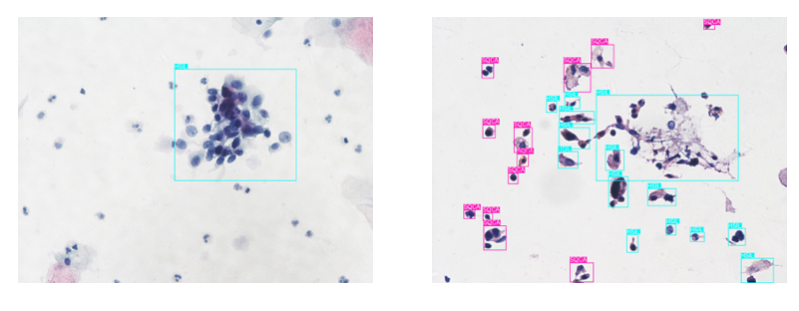
\includegraphics[width=0.5\paperwidth]{TCT/HSIL-SQCA.png}
              \caption{HSIL与SQCA两个类别的特征,左图为HSIL,右图为SQCA。全片与部分视野的大小对比。}
              \label{HSIL-SQCA}
          \end{figure}
\end{enumerate}
\par 由此,为了减少医生的工作量,避免诊断过程中因为人为原因造成遗漏等问题,并进一步提高诊断结果的准确性,我们亟需计算机的辅助诊断方法以实现快速、准确的宫颈癌筛查。

\section{国内外研究现状}
\par 目前国内外通过计算机辅助医生进行宫颈TCT检测的方法主要分为病变细胞分类、病变细胞检测、病变部位分割三个部分。
\par 病变细胞分类主要是指仅给出输入视野中细胞的综合病变等级,一般会根据病变细胞的状况评定为在视野中出现的最高病变等级或者次高级。

\begin{figure}[h]
    \centering
    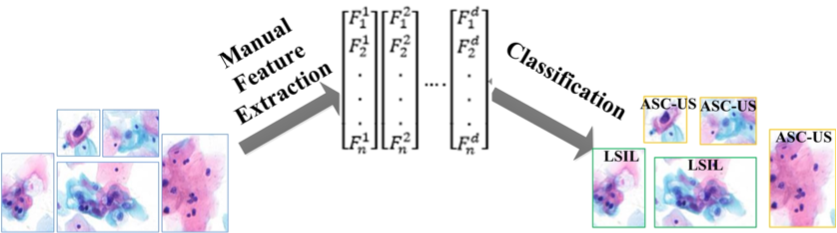
\includegraphics[width=0.5\paperwidth]{TCT/分类样例.png}
    \caption{病变细胞分类样例图片,输入图片经过提取特征等处理后由计算机判断图片所属的病变等级}
    \label{分类样例}
\end{figure}
\par 病变细胞检测则是要求以矩形框的方式标注出视野内的病变细胞并给出病变等级,相较病变细胞分类任务而言,评定整个视野的综合病变等级的任务由医生完成。在病变细胞检测的任务中,计算机应当标注出所有病变细胞的位置并给每个病变细胞评定病变等级。

\begin{figure}[h]
    \centering
    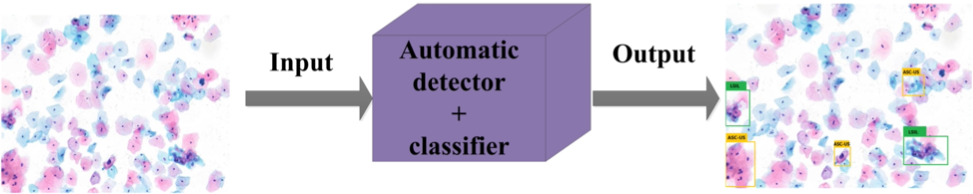
\includegraphics[width=0.5\paperwidth]{TCT/检测样例.png}
    \caption{病变细胞检测样例图片,输入图片经过提取特征等处理后由计算机检测图片所有的病变细胞并判定其所属的病变等级}
    \label{检测样例}
\end{figure}
\par 病变细胞分割则是在病变细胞检测的基础上,要求以像素级的精度标注出病变细胞的范围。病变细胞分割的任务中,计算机标注病变细胞位置的结果应当更为精确。

\begin{figure}[h]
    \centering
    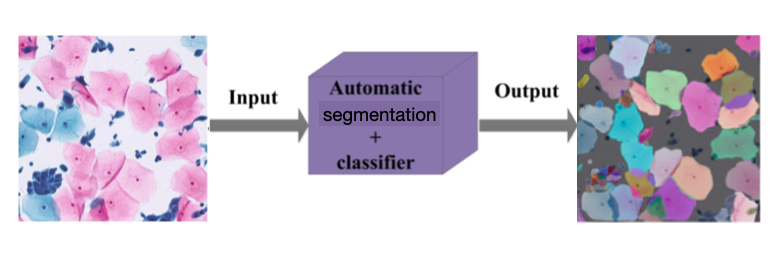
\includegraphics[width=0.5\paperwidth]{TCT/分割样例.png}
    \caption{分割样例图片,左图为样例图片,右图为样例图片的分割结果}
    \label{分割样例}
\end{figure}

\subsection{研究方向及进展}

\subsubsection{病变细胞分类与分割}
\par 在临床实践中,医生主要依据细胞核与细胞质的比例,细胞核的大小,细胞核的形状以及核膜的异常变化来判定病变的宫颈细胞,以及区分它们的种类。因此,有许多研究\cite{zhang2014segmentation}\cite{zhang2017graph}\cite{lee2016segmentation}通过分割细胞或细胞的某些部分(细胞核、细胞质),并依据临床上的判定规则完成病变细胞的分类任务。但是由于不同种类细胞的形态差异较大、细胞之间的重叠问题可能比较严重以及细胞质边界可能不够清晰等问题,细胞以及细胞成分的分割依然是一个尚未被很好解决的问题。因此,这类方法往往不能让人满意。
\par 而在另一方面,也有许多研究\cite{marinakis2009pap}\cite{phoulady2016automatic}通过手工设计大量的特征试图捕捉细胞核和细胞质的形态特征,再将这些特征经过特征选择或者降维处理之后输入到各种分类器中(如,随机森林、SVM、神经网络等)来完成分类任务。但是,上述的手工设计的特征往往依赖于细胞或细胞组成成分的分割结果,而且这些手工设计的特征完全来自于当前医学对于宫颈细胞学的认知,因此,此类方法的发展会受到医学发展的限制。
\subsubsection{病变细胞检测}
\par 近期,病变细胞检测方向的研究主要是基于卷积神经网络进行的。例如,Ma等\cite{ma2020macd}中设计了新的MACD R-CNN网络,通过在Mask R-CNN的不同分类分支中使用不同的roi提取出一个细胞核特征变形的特征图,将这种特征图与固定roi的特征通过注意力机制合并,最后通过加入更深的卷积层深度提高了检测的精度;Xiang等\cite{xiang2020novel}基于YOLOv3级联了一个额外的特定任务分类器,还通过平滑噪声标签的分布来处理可能存在的不可靠标注,最终提高了宫颈细胞水平诊断的平均精度;Liang等\cite{liang2018comparison}通过将图像提案与各类别的参考样本进行比较,来对图像提案进行分类,并且从数据中学习背景的参考样本,而不是通过一些启发式规则手工选择参考样本,这种方法在小数据集上相较与基准模型会有明显提升,在中等数据集上会略有提升;Li等\cite{li2019detection}提出了一种基于多语义标签和形态信息分析相结合的目标检测和分类方法,该方法以ResNet101作为骨干网络时可以在LBC数据集上取得66.98\%的平均精度;Liu等\cite{liu2018multitask}使用VGG16迁移学习,并用一种面向任务的基于先验框的网络将产生潜在的感兴趣区域,最后使用全卷积网络来估计细胞的位置并将其分类,这种方法在保持性能和计算效率之间取得了良好的平衡,相较于YOLO和Faster R-CNN它拥有更好的精度和更快的速度,例如,这种方法的耗时只有Faster R-CNN的一半。
\par 除此之外,由于卷积神经网络的学习往往需要大量的标注数据,而TCT图像的标注结果是由专业的医师来完成的,那么获取大量的数据就会带来高额的成本,因此也有许多研究\cite{zhou2020deep}\cite{yu2019uncertainty}通过一些半监督的方法来利用大量无标注信息的图像促进网络的学习。Zhou等\cite{zhou2020deep}提出了一种新的带扰动敏感样本挖掘的掩码引导的均值教师框架,该框架在训练过程中由教师和学生网络组成。在小扰动条件下,两个网络在特征和语义层面上保持一致。从教师网络对样本的预测来构建可靠的伪标签以优化学生网络。他们设计了一个新的策略来估计每个提案对扰动的敏感性,并从大量的可能样本中选择最具信息量的样本,以促进快速有效的语义提取。此外,为了消除背景区域不可避免的噪声,他们希望以预测出的分割掩模作为指导以加强前景区域的特征蒸馏。与仅使用已有标注数据的监督方法相比,该方法的性能有显著提高;Yu等\cite{yu2019uncertainty}提出了一种新的不确定性感知的半监督框架,该框架可以有效地利用未标记的数据,鼓励在不同扰动下对相同输入进行一致的预测。具体来说,该框架由一个学生模型和一个教师模型组成,学生模型通过最小化分割损失和一致性损失对教师模型的目标进行学习。他们设计了一种新的不确定性感知方案,使学生模型能够利用不确定性信息逐步学到有意义的、可靠的目标。实验表明,该方法通过合并未标记的数据获得了较高的性能。
\par 目前病变细胞检测方面相关的论文、其所使用的方法、数据集以及最终效果(部分)如\ref{检测论文}:
\begin{table}[htbp]
    \center
    \tiny
    \caption{病变细胞检测论文汇总}
    \begin{tabular}{p{120pt}p{100pt}p{85pt}p{35pt}}
        \hline
        论文                                                             & 模型                         & 数据                       & 效果(mAP) \\
        \hline
        MACD R-CNN\cite{ma2020macd}                                      & 基于mask R-CNN 的 MACD R-CNN & Herlev 数据集              & -           \\
        Automation-Assisted Reading Method\cite{xiang2020novel}          & YOLO V3 和额外的分类器       & 私有数据12909 例,10个类别 & 0.634       \\
        Detection in the Limited Data Scenario\cite{liang2018comparison} & Faster R-CNN + FPN           & 私有数据7086例,11个类别   & 0.263       \\
        Detection and Classification of Cells\cite{li2019detection}      & Faster R-CNN                 & 680例,6个类别             & -           \\
        Multitask Learning for Recognition\cite{liu2018multitask}        & VGG16                        & 73 例                      & -           \\
        DCCL\cite{zhang2019dccl}                                         & Faster R-CNN,RetinaNet      & DCCL公开数据               & -           \\
        \hline
    \end{tabular}
    \label{检测论文}
\end{table}

\subsection{存在问题}
\subsubsection{染色导致的色彩差异}
\par TCT检查的视野中细胞各个部分的颜色并不是细胞本身的颜色,而是染色剂染色之后的颜色。因此,即使是同样的细胞部位、同样的病变程度,也可能因为染色剂的不同而呈现出不同的颜色状态。不仅如此,输入到计算机中的视野图片并不一定是TCT检查刚刚做完时的视野图片,而染色剂会随着时间慢慢褪色。不同染色剂品牌,不同颜色的染色剂都会有不同的褪色速率,因此,即使是同一份TCT涂片也可能因为输入计算机系统的时间不同而表现出不同的色彩状态。
\begin{figure}[h]
    \centering
    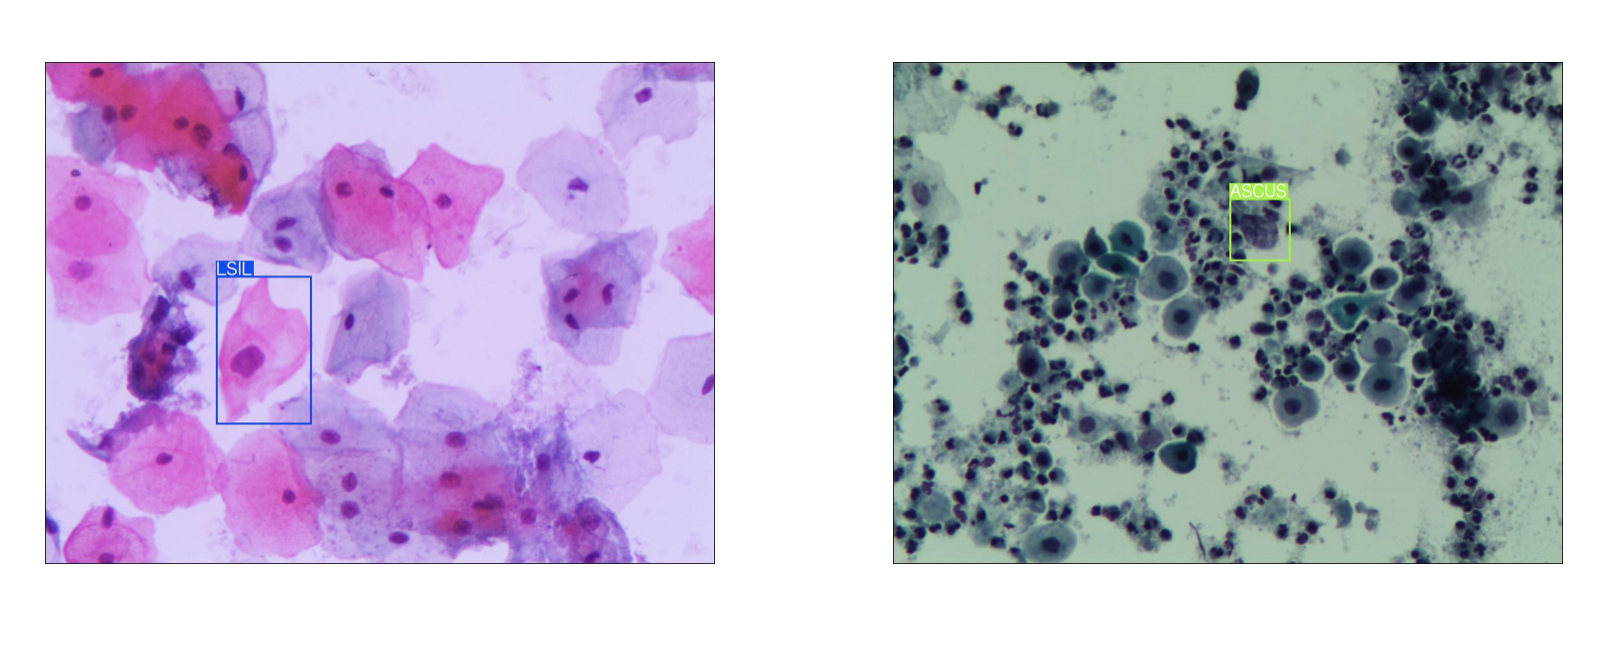
\includegraphics[width=0.5\paperwidth]{TCT/色彩差异.png}
    \caption{不同样片之间由于使用的染色剂不同、褪色时间不同等原因表现出完全不同的色彩差异}
    \label{色彩差异}
\end{figure}
\subsubsection{单细胞与细胞簇的形态差异}
\par 医生在标注病变细胞框的时候,如果病变细胞是单个存在的、周围没有其他细胞的状态,那么医生会给该细胞单独标注一个框。但是,如果病变细胞聚集在一起形成了一个很大的细胞簇,那么病变细胞之间的界限会变得十分糢糊,只能选择标注一个很大的框将整个细胞簇框住。这就导致了同一种类标签的标注框有着两种不同的含义——既可以是单个的病变细胞,也可以是一整个病变细胞簇,而二者在形态上有着巨大的差异。
\par 例如,由于不论是病变细胞还是正常细胞细胞核往往在形态上处在整个细胞中心的位置,那么单个细胞对应的框的中心一般来说就是这个细胞的细胞核,因此从该处往往可以获得细胞核的形态特征。换句话说,如果网络发现了细胞核的形态特征,就可以将该点作为检测框的中心的进行预测。但是,如果框中的是一个大的细胞簇那么其中心就不再是明显的细胞核的特征了。而细胞核的形态特征又是判断病变与否已经病变种类的相当关键的特征,这就导致网络的学习过程中可能遇到难以学习的特征形态。与此类似的,单个细胞框的周围会是细胞质边界的特征,这也是判断病变细胞的一个重要特征,但是细胞簇的边缘是多个细胞聚集在一起时组成的形状,因为细胞是经过混匀的,这一形态信息完全由混匀过程决定可以认为是随机的,这对判断细胞的病变程度毫无意义。
\par 此外,单个细胞与细胞簇的界限并没有那么明显。例如,医生在标注框的时候,会遇到两三个细胞挨在一起的情况,这种情况下可以说为每个细胞单独标注框和将这两三个细胞视作一个细胞簇只标注一个框都是合理的。但这就给网络的学习带来了很大的难度——网络不仅要学会如何判断病变细胞,还需要学会制作训练用数据集的医生对于上述情况的偏好情况。而事实上,由于数据的标注由不止一位医生完成,往往每位医生对都上述情况会有不同的偏好,因此,网络可能根本无法学习到这一规律。这一问题严重地阻碍了网络的学习过程,然而,在实践中,我们往往并不关注病变细胞是有单独的框还是由一个框标注出来的,我们更关心病变细胞的召回率和病变等级判定的准确率。
\begin{figure}[h]
    \centering
    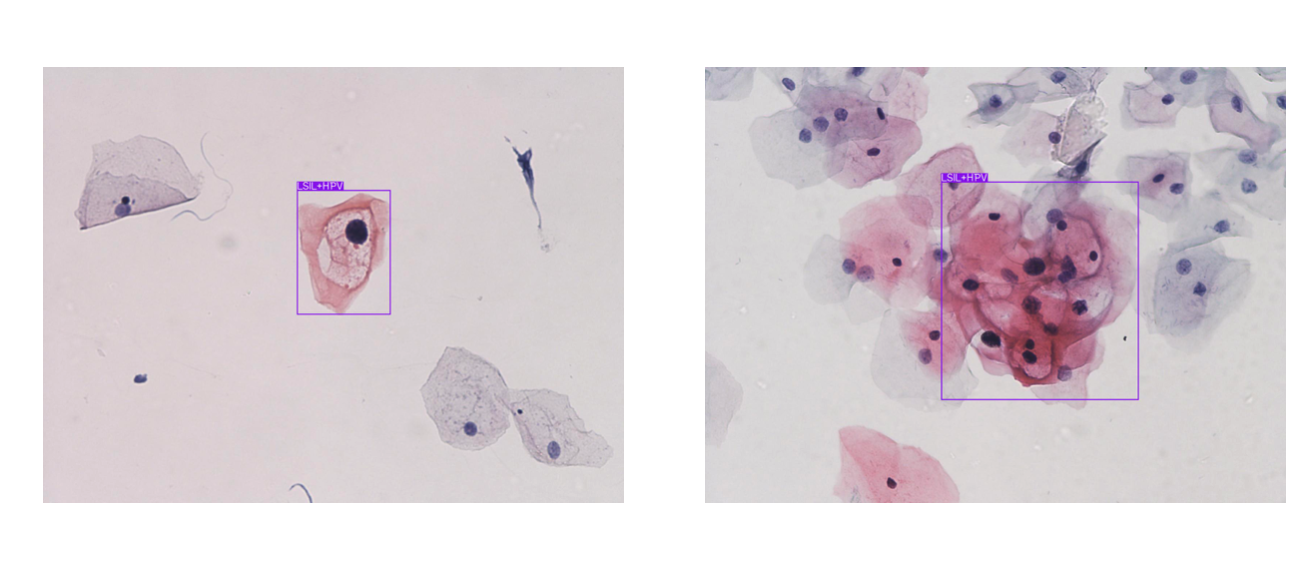
\includegraphics[width=0.5\paperwidth]{TCT/single_multi.png}
    \caption{单个病变细胞与病变细胞簇形态差异比较,左图为单个病变细胞,右图为许多病变细胞形成的细胞簇,两图中的病变细胞均为统一病变等级,但是由于细胞数目不同而具有完全不同的形态特征}
    \label{形态差异}
\end{figure}
\subsubsection{放大倍率不一致}
\par TCT检查的图片都是经过显微镜放大的,所以图片中细胞的绝对大小并没有实际的意义,甚至这一大小的变换还会为网络的学习带来阻碍。例如,涂片中可能出现一种叫做炎细胞的正常细胞,它相比入一般细胞会小得多,医生在做诊断时可以自然地忽略它,但是它的形态特征在放大之后与最高等级的病变细胞——鳞癌细胞的形态特征十分相近。他们的区别只是炎细胞相较与正常细胞非常小,而鳞癌细胞具有正常细胞的大小尺度。现有的深度学习方法主要通过FPN来生成各种尺度的图像金字塔来处理这种尺度变换的问题,但是,这种方法更适合用来检测尺度大小不确定的目标,对于形态特征相近只有尺度不同的目标,这种方式反而会影响网络的训练。
\begin{figure}[h]
    \centering
    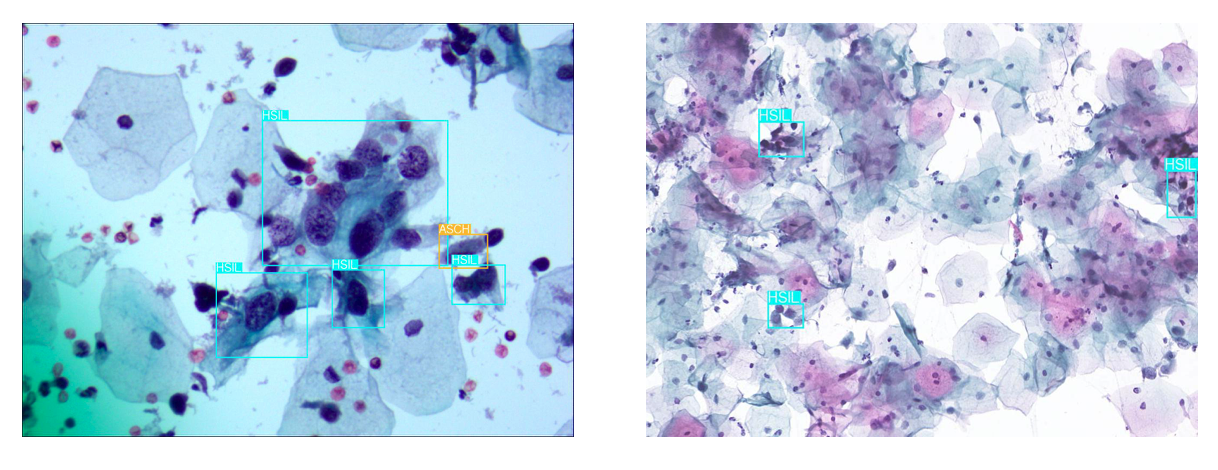
\includegraphics[width=0.5\paperwidth]{TCT/scale.png}
    \caption{不同图片之间放大倍率有着较大的差距,左图中的正常细胞大小相较右图中大得多,而实际上正常细胞的大小应当是一致的,所以左图放大倍率应当比右图高很多}
    \label{倍率差异}
\end{figure}
\section{研究展望}
\par 目前,已有部分工作致力于解决关于不同染色剂等问题导致的色彩差异问题,由此,我们主要关注单细胞与细胞簇之间的形态差异和放大倍率不一致这两个问题。我们望通过不同的方法尝试解决或者缓解上述问题对网络学习的影响。

\subsection{单细胞与细胞簇的形态差异}
\par 由于单个细胞和细胞簇在形态上的巨大差异以及它们之间的语义差异,如果通过同一个网络同时捕捉这两者的形态特征,可能会引起模型学习过程中的特征冲突。由此,我们希望通过对数据标注的重新整理和重新标注区分出单个细胞的框和细胞簇对应的框,并分别使用不同的网络结构来分别预测他们,以此,促进网络捕捉相对应类别的形态特征,促进网络的学习过程。

\subsection{放大倍率不一致}
\par 医生在标注图片、诊断病例的过程中往往会依靠视野中的正常细胞大小来作为基准,以此来判断病变细胞的大小。其中,正常细胞的细胞核大小和细胞质大小是十分重要的判断依据,医生主要通过对比病变细胞与正常细胞的细胞核大小、细胞质大小来判定病变程度。因此,我们希望模仿医生判断的过程,让网络可以先识别一些正常细胞,然后依据正常细胞的形态、尺寸信息来帮助病变细胞的识别与类别判定。

\newpage
\begingroup
\linespread{1}
\printbibliography[title={参考文献}]
\endgroup
